% Options for packages loaded elsewhere
\PassOptionsToPackage{unicode}{hyperref}
\PassOptionsToPackage{hyphens}{url}
%
\documentclass[
]{article}
\usepackage{amsmath,amssymb}
\usepackage{lmodern}
\usepackage{iftex}
\ifPDFTeX
  \usepackage[T1]{fontenc}
  \usepackage[utf8]{inputenc}
  \usepackage{textcomp} % provide euro and other symbols
\else % if luatex or xetex
  \usepackage{unicode-math}
  \defaultfontfeatures{Scale=MatchLowercase}
  \defaultfontfeatures[\rmfamily]{Ligatures=TeX,Scale=1}
\fi
% Use upquote if available, for straight quotes in verbatim environments
\IfFileExists{upquote.sty}{\usepackage{upquote}}{}
\IfFileExists{microtype.sty}{% use microtype if available
  \usepackage[]{microtype}
  \UseMicrotypeSet[protrusion]{basicmath} % disable protrusion for tt fonts
}{}
\makeatletter
\@ifundefined{KOMAClassName}{% if non-KOMA class
  \IfFileExists{parskip.sty}{%
    \usepackage{parskip}
  }{% else
    \setlength{\parindent}{0pt}
    \setlength{\parskip}{6pt plus 2pt minus 1pt}}
}{% if KOMA class
  \KOMAoptions{parskip=half}}
\makeatother
\usepackage{xcolor}
\usepackage[margin=1in]{geometry}
\usepackage{color}
\usepackage{fancyvrb}
\newcommand{\VerbBar}{|}
\newcommand{\VERB}{\Verb[commandchars=\\\{\}]}
\DefineVerbatimEnvironment{Highlighting}{Verbatim}{commandchars=\\\{\}}
% Add ',fontsize=\small' for more characters per line
\usepackage{framed}
\definecolor{shadecolor}{RGB}{248,248,248}
\newenvironment{Shaded}{\begin{snugshade}}{\end{snugshade}}
\newcommand{\AlertTok}[1]{\textcolor[rgb]{0.94,0.16,0.16}{#1}}
\newcommand{\AnnotationTok}[1]{\textcolor[rgb]{0.56,0.35,0.01}{\textbf{\textit{#1}}}}
\newcommand{\AttributeTok}[1]{\textcolor[rgb]{0.77,0.63,0.00}{#1}}
\newcommand{\BaseNTok}[1]{\textcolor[rgb]{0.00,0.00,0.81}{#1}}
\newcommand{\BuiltInTok}[1]{#1}
\newcommand{\CharTok}[1]{\textcolor[rgb]{0.31,0.60,0.02}{#1}}
\newcommand{\CommentTok}[1]{\textcolor[rgb]{0.56,0.35,0.01}{\textit{#1}}}
\newcommand{\CommentVarTok}[1]{\textcolor[rgb]{0.56,0.35,0.01}{\textbf{\textit{#1}}}}
\newcommand{\ConstantTok}[1]{\textcolor[rgb]{0.00,0.00,0.00}{#1}}
\newcommand{\ControlFlowTok}[1]{\textcolor[rgb]{0.13,0.29,0.53}{\textbf{#1}}}
\newcommand{\DataTypeTok}[1]{\textcolor[rgb]{0.13,0.29,0.53}{#1}}
\newcommand{\DecValTok}[1]{\textcolor[rgb]{0.00,0.00,0.81}{#1}}
\newcommand{\DocumentationTok}[1]{\textcolor[rgb]{0.56,0.35,0.01}{\textbf{\textit{#1}}}}
\newcommand{\ErrorTok}[1]{\textcolor[rgb]{0.64,0.00,0.00}{\textbf{#1}}}
\newcommand{\ExtensionTok}[1]{#1}
\newcommand{\FloatTok}[1]{\textcolor[rgb]{0.00,0.00,0.81}{#1}}
\newcommand{\FunctionTok}[1]{\textcolor[rgb]{0.00,0.00,0.00}{#1}}
\newcommand{\ImportTok}[1]{#1}
\newcommand{\InformationTok}[1]{\textcolor[rgb]{0.56,0.35,0.01}{\textbf{\textit{#1}}}}
\newcommand{\KeywordTok}[1]{\textcolor[rgb]{0.13,0.29,0.53}{\textbf{#1}}}
\newcommand{\NormalTok}[1]{#1}
\newcommand{\OperatorTok}[1]{\textcolor[rgb]{0.81,0.36,0.00}{\textbf{#1}}}
\newcommand{\OtherTok}[1]{\textcolor[rgb]{0.56,0.35,0.01}{#1}}
\newcommand{\PreprocessorTok}[1]{\textcolor[rgb]{0.56,0.35,0.01}{\textit{#1}}}
\newcommand{\RegionMarkerTok}[1]{#1}
\newcommand{\SpecialCharTok}[1]{\textcolor[rgb]{0.00,0.00,0.00}{#1}}
\newcommand{\SpecialStringTok}[1]{\textcolor[rgb]{0.31,0.60,0.02}{#1}}
\newcommand{\StringTok}[1]{\textcolor[rgb]{0.31,0.60,0.02}{#1}}
\newcommand{\VariableTok}[1]{\textcolor[rgb]{0.00,0.00,0.00}{#1}}
\newcommand{\VerbatimStringTok}[1]{\textcolor[rgb]{0.31,0.60,0.02}{#1}}
\newcommand{\WarningTok}[1]{\textcolor[rgb]{0.56,0.35,0.01}{\textbf{\textit{#1}}}}
\usepackage{longtable,booktabs,array}
\usepackage{calc} % for calculating minipage widths
% Correct order of tables after \paragraph or \subparagraph
\usepackage{etoolbox}
\makeatletter
\patchcmd\longtable{\par}{\if@noskipsec\mbox{}\fi\par}{}{}
\makeatother
% Allow footnotes in longtable head/foot
\IfFileExists{footnotehyper.sty}{\usepackage{footnotehyper}}{\usepackage{footnote}}
\makesavenoteenv{longtable}
\usepackage{graphicx}
\makeatletter
\def\maxwidth{\ifdim\Gin@nat@width>\linewidth\linewidth\else\Gin@nat@width\fi}
\def\maxheight{\ifdim\Gin@nat@height>\textheight\textheight\else\Gin@nat@height\fi}
\makeatother
% Scale images if necessary, so that they will not overflow the page
% margins by default, and it is still possible to overwrite the defaults
% using explicit options in \includegraphics[width, height, ...]{}
\setkeys{Gin}{width=\maxwidth,height=\maxheight,keepaspectratio}
% Set default figure placement to htbp
\makeatletter
\def\fps@figure{htbp}
\makeatother
\setlength{\emergencystretch}{3em} % prevent overfull lines
\providecommand{\tightlist}{%
  \setlength{\itemsep}{0pt}\setlength{\parskip}{0pt}}
\setcounter{secnumdepth}{5}
\newlength{\cslhangindent}
\setlength{\cslhangindent}{1.5em}
\newlength{\csllabelwidth}
\setlength{\csllabelwidth}{3em}
\newlength{\cslentryspacingunit} % times entry-spacing
\setlength{\cslentryspacingunit}{\parskip}
\newenvironment{CSLReferences}[2] % #1 hanging-ident, #2 entry spacing
 {% don't indent paragraphs
  \setlength{\parindent}{0pt}
  % turn on hanging indent if param 1 is 1
  \ifodd #1
  \let\oldpar\par
  \def\par{\hangindent=\cslhangindent\oldpar}
  \fi
  % set entry spacing
  \setlength{\parskip}{#2\cslentryspacingunit}
 }%
 {}
\usepackage{calc}
\newcommand{\CSLBlock}[1]{#1\hfill\break}
\newcommand{\CSLLeftMargin}[1]{\parbox[t]{\csllabelwidth}{#1}}
\newcommand{\CSLRightInline}[1]{\parbox[t]{\linewidth - \csllabelwidth}{#1}\break}
\newcommand{\CSLIndent}[1]{\hspace{\cslhangindent}#1}
\ifLuaTeX
  \usepackage{selnolig}  % disable illegal ligatures
\fi
\IfFileExists{bookmark.sty}{\usepackage{bookmark}}{\usepackage{hyperref}}
\IfFileExists{xurl.sty}{\usepackage{xurl}}{} % add URL line breaks if available
\urlstyle{same} % disable monospaced font for URLs
\hypersetup{
  pdftitle={Check your outliers! An accessible introduction to identifying statistical outliers in R with easystats},
  hidelinks,
  pdfcreator={LaTeX via pandoc}}

\title{Check your outliers! An accessible introduction to identifying statistical outliers in R with \emph{easystats}}
\author{}
\date{\vspace{-2.5em}}

\begin{document}
\maketitle

\hypertarget{abstract}{%
\section{Abstract}\label{abstract}}

xyz

\hypertarget{introduction}{%
\section{Introduction}\label{introduction}}

The improper handling of outliers can substantially affect statistical model estimations, thus contributing to false positives (Simmons et al., 2011) but almost certainly to false negatives as well. It is thus essential to address this problem in a thoughtful manner. Fortunately, guidelines exist in this regard. Yet, especially in the field of psychology, many researchers still do not treat outliers in a consistent manner or do so using inappropriate strategies (Leys et al., 2013; Simmons et al., 2011).

One possible reason is that researchers do not know of existing recommendations or currently available software options for their implementation. In this paper, we show how to follow current recommendations for statistical outlier detection (SOD) using R and the \{performance\} package (Lüdecke et al., 2021) from the \emph{easystats} ecosystem.

\hypertarget{identifying-outliers}{%
\section{Identifying Outliers}\label{identifying-outliers}}

Although many researchers attempt to identify outliers with measures based on the mean (e.g., \emph{z} scores), those methods are problematic because the mean and standard deviation themselves are not robust to the influence of outliers and they assume a normal distribution. Therefore, current guidelines recommend using robust methods to identify outliers, such as those relying on the median as opposed to the mean (Leys et al., 2013, 2019).

Nonetheless, which exact outlier method to use depends on several factors, like the statistical test of interest. When using a regression model, for example, the most relevant information will be regarding observations that do not fit well with the model, known as model-based outliers. When no method is readily available to detect model-based outliers, such as for structural equation modelling (SEM), looking for multivariate outliers may be of relevance. Finally, for simple tests (\emph{t} tests or correlations) that compare values of the same variable, it can make sense to check for univariate outliers. However, univariate methods can give false positives since \emph{t} tests and correlations, ultimately, are also models/multivariable statistics {[}REF?{]}. They are in this sense more limited, but we show them nonetheless for educational purposes. In the following section, we will go through each of the mentioned methods.

Regardless of the method used, we remind readers that transparency is key (Leys et al., 2019). Researchers should commit (ideally in a preregistration) to an outlier decision tree before collecting the data. They should report in the paper their decisions and details of their methods, as well as any deviation from their original plan. These transparency practices can help reduce false positives due to excessive researchers' degrees of freedom (choice flexibility throughout the analysis).

\hypertarget{univariate-outliers}{%
\subsection{Univariate Outliers}\label{univariate-outliers}}

For univariate outliers, it is recommended to use the median along the Median Absolute Deviation (MAD), which is more robust than the interquartile range or the mean and its standard deviation (Leys et al., 2013, 2019). The MAD can be calculated as follow:

\[
MAD = b M_i(|x_i-M_j(x_j)|)
\]
Where \(b\) is a scaler, often set to \(1/\left(\Phi ^{-1}(3/4)\right)\approx 1.4826\).

In \{performance\}'s \texttt{check\_outliers()}, one can use this approach with \texttt{method\ =\ "zscore\_robust"}. Although Leys et al. (2013) suggest a default threshold of 2.5 and Leys et al. (2019) a threshold of 3, for consistency with other outlier detection methods, \{performance\} uses a less conservative threshold of 3.09 by default. That is, data points will be flagged as outliers if they go beyond +/- 3.09 MAD. Users can adjust this threshold using the \texttt{threshold} argument.

Example:

\begin{Shaded}
\begin{Highlighting}[]
\FunctionTok{library}\NormalTok{(performance)}

\CommentTok{\# create some fake outliers and an ID column}
\NormalTok{data }\OtherTok{\textless{}{-}} \FunctionTok{rbind}\NormalTok{(mtcars[}\DecValTok{1}\SpecialCharTok{:}\DecValTok{4}\NormalTok{], }\DecValTok{42}\NormalTok{, }\DecValTok{55}\NormalTok{)}
\NormalTok{data }\OtherTok{\textless{}{-}} \FunctionTok{cbind}\NormalTok{(}\AttributeTok{car =} \FunctionTok{row.names}\NormalTok{(data), data)}

\NormalTok{x }\OtherTok{\textless{}{-}} \FunctionTok{check\_outliers}\NormalTok{(data, }\AttributeTok{method =} \StringTok{"zscore\_robust"}\NormalTok{, }\AttributeTok{ID =} \StringTok{"car"}\NormalTok{)}
\NormalTok{x}
\end{Highlighting}
\end{Shaded}

\begin{verbatim}
#> 2 outliers detected: cases 33, 34.
#> - Based on the following method and threshold: zscore_robust (3.09).
#> - For variables: mpg, cyl, disp, hp.
#> 
#> -----------------------------------------------------------------------------
#> The following observations were considered outliers for two or more variables 
#> by at least one of the selected methods: 
#> 
#>   Row car n_Zscore_robust
#> 1  33  33               2
#> 2  34  34               2
#> 
#> -----------------------------------------------------------------------------
#> Outliers per variable (zscore_robust): 
#> 
#> $mpg
#>    Row car Distance_Zscore_robust
#> 33  33  33               3.709699
#> 34  34  34               5.848328
#> 
#> $cyl
#>    Row car Distance_Zscore_robust
#> 33  33  33               12.14083
#> 34  34  34               16.52502
\end{verbatim}

All \texttt{check\_outliers()} output objects possess a \texttt{plot()} method, meaning it is also possible to visualize the outliers:



\begin{Shaded}
\begin{Highlighting}[]
\FunctionTok{library}\NormalTok{(see)}
\FunctionTok{plot}\NormalTok{(x)}
\end{Highlighting}
\end{Shaded}

\begin{figure}
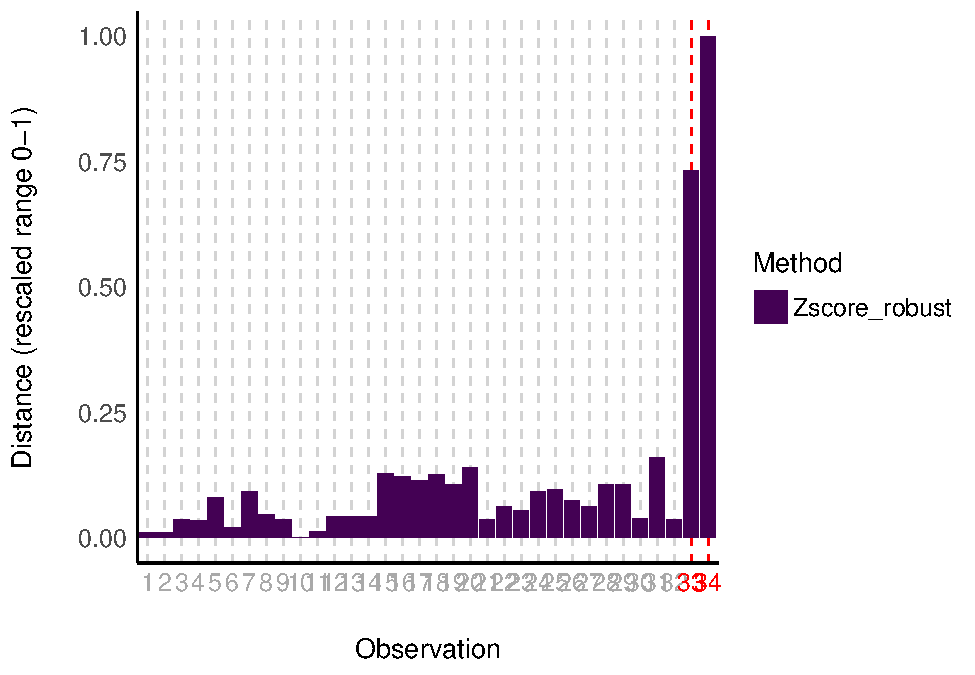
\includegraphics[width=1\linewidth]{paper_files/figure-latex/univariate-1} \caption{Visual depiction of outliers using the robust \emph{z} score method.}\label{fig:univariate}
\end{figure}

\hypertarget{multivariate-outliers}{%
\subsection{Multivariate Outliers}\label{multivariate-outliers}}

For multivariate outliers, it is recommended to use the Minimum Covariance Determinant, a robust version of the Mahalanobis distance (MCD, Leys et al., 2019). In \{performance\}'s \texttt{check\_outliers()}, one can use this approach with \texttt{method\ =\ "mcd"}. The MCD can be calculated as follow (Hubert et al., 2018):

\[
MATTHS_{gohere}^{andB}
\]

\textbf{{[}mattansb can you add some maths here; perhaps from Hubert et al. (2018)? \url{https://doi.org/10.1002/wics.1421}{]}}

Example:



\begin{Shaded}
\begin{Highlighting}[]
\NormalTok{x }\OtherTok{\textless{}{-}} \FunctionTok{check\_outliers}\NormalTok{(data, }\AttributeTok{method =} \StringTok{"mcd"}\NormalTok{)}
\NormalTok{x}
\end{Highlighting}
\end{Shaded}

\begin{verbatim}
#> 6 outliers detected: cases 15, 16, 17, 31, 33, 34.
#> - Based on the following method and threshold: mcd (18.47).
#> - For variables: mpg, cyl, disp, hp.
\end{verbatim}

\begin{Shaded}
\begin{Highlighting}[]
\FunctionTok{plot}\NormalTok{(x)}
\end{Highlighting}
\end{Shaded}

\begin{figure}
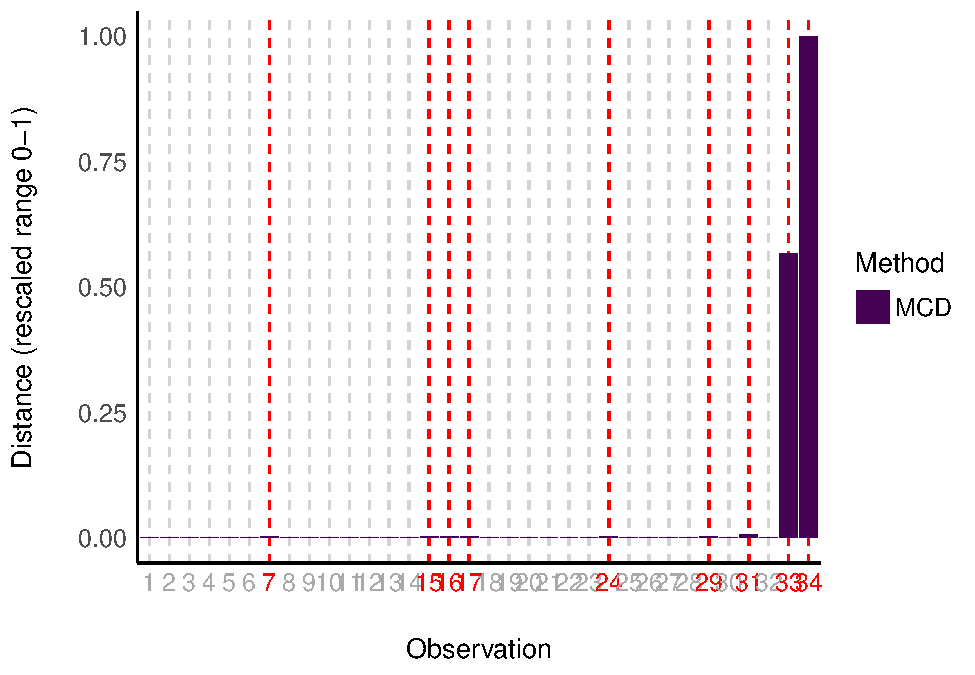
\includegraphics[width=1\linewidth]{paper_files/figure-latex/multivariate-1} \caption{Visual depiction of outliers using the Minimum Covariance Determinant (MCD) method, a robust version of the Mahalanobis distance.}\label{fig:multivariate}
\end{figure}

\hypertarget{model-based-outliers}{%
\subsection{Model-Based Outliers}\label{model-based-outliers}}

{[}FIND REFERENCES TO SUPPORT MODEL-BASED OUTLIER DETECTION ABOVE ALL OTHER METHODS!!{]}

Something something\ldots{} what is leverage\ldots{} why we should care if few observations have (relatively) strong leverage (answer: they are suspect of biasing our estimates!).

When working with regression models, model-based outliers can be detected using \texttt{check\_outliers()} by specifying \texttt{method\ =\ "cook"} (or \texttt{method\ =\ "pareto"} for Bayesian models). The Cook's distance can be calculated as follow:

\[
MATTHS_{gohere}^{andB}
\]

\textbf{{[}mattansb can you add some maths here?{]}}

Example:



\begin{Shaded}
\begin{Highlighting}[]
\NormalTok{model }\OtherTok{\textless{}{-}} \FunctionTok{lm}\NormalTok{(disp }\SpecialCharTok{\textasciitilde{}}\NormalTok{ mpg }\SpecialCharTok{*}\NormalTok{ hp, }\AttributeTok{data =}\NormalTok{ data)}
\NormalTok{x }\OtherTok{\textless{}{-}} \FunctionTok{check\_outliers}\NormalTok{(model, }\AttributeTok{method =} \StringTok{"cook"}\NormalTok{)}
\NormalTok{x}
\end{Highlighting}
\end{Shaded}

\begin{verbatim}
#> 2 outliers detected: cases 31, 34.
#> - Based on the following method and threshold: cook (0.86).
#> - For variable: (Whole model).
\end{verbatim}

\begin{Shaded}
\begin{Highlighting}[]
\FunctionTok{plot}\NormalTok{(x)}
\end{Highlighting}
\end{Shaded}

\begin{figure}
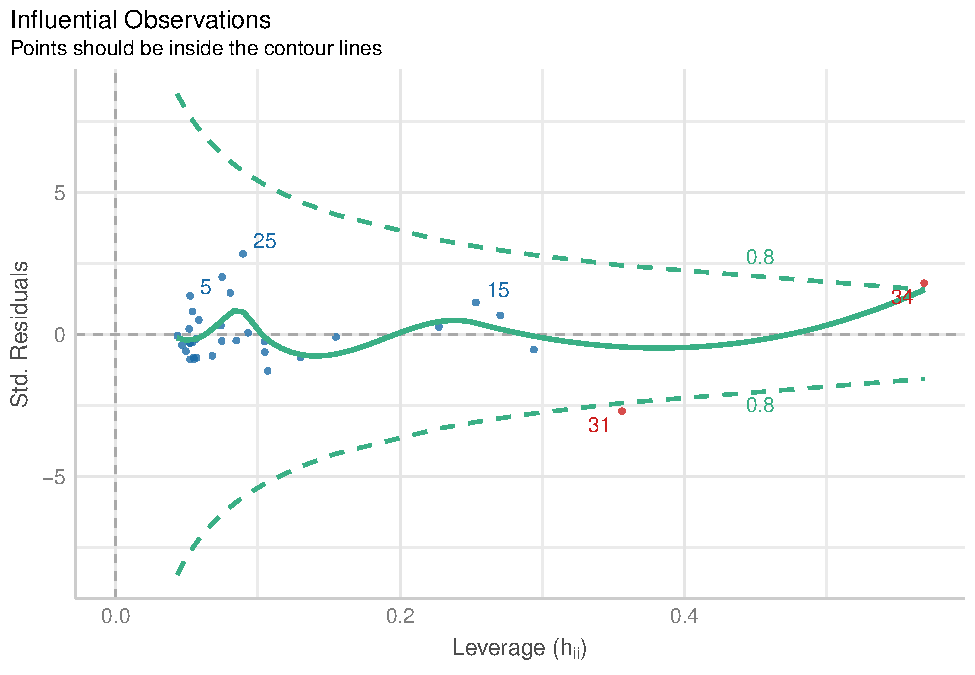
\includegraphics[width=1\linewidth]{paper_files/figure-latex/model-1} \caption{Visual depiction of outliers using Cook's distance.}\label{fig:model}
\end{figure}

\hypertarget{multiple-methods}{%
\subsection{Multiple methods}\label{multiple-methods}}

An alternative approach suggested by easystats is to combine several methods. This approach computes a composite outlier score, formed of the average of the binary (0 or 1) results of each method. It represents the probability that each observation is classified as an outlier by at least one method. The default decision rule classifies rows with composite outlier scores superior or equal to 0.5 as outlier observations (i.e., that were classified as outliers by at least half of the methods). In \{performance\}'s \texttt{check\_outliers()}, one can use this approach by including all desired methods in the corresponding argument.

Example:



\begin{Shaded}
\begin{Highlighting}[]
\NormalTok{x }\OtherTok{\textless{}{-}} \FunctionTok{check\_outliers}\NormalTok{(}
\NormalTok{  data,}
  \AttributeTok{method =} \FunctionTok{c}\NormalTok{(}\StringTok{"zscore\_robust"}\NormalTok{, }\StringTok{"iqr"}\NormalTok{, }\StringTok{"mcd"}\NormalTok{, }\StringTok{"ics"}\NormalTok{),}
  \AttributeTok{ID =} \StringTok{"car"}
\NormalTok{)}
\NormalTok{x}
\end{Highlighting}
\end{Shaded}

\begin{verbatim}
#> 3 outliers detected: cases 31, 33, 34.
#> - Based on the following methods and thresholds: zscore_robust (3.09),
#>   iqr (1.7), mcd (18.47), ics (0).
#> - For variables: mpg, cyl, disp, hp.
#> 
#> Note: Outliers were classified as such by at least half of the selected methods. 
#> 
#> -----------------------------------------------------------------------------
#> The following observations were considered outliers for two or more variables 
#> by at least one of the selected methods: 
#> 
#>   Row                 car n_Zscore_robust n_IQR          n_MCD          n_ICS
#> 1  33                  33               2     2 (Multivariate) (Multivariate)
#> 2  34                  34               2     2 (Multivariate) (Multivariate)
#> 3  31       Maserati Bora               0     1 (Multivariate) (Multivariate)
#> 4   7          Duster 360               0     0 (Multivariate)              0
#> 5  15  Cadillac Fleetwood               0     0 (Multivariate)              0
#> 6  16 Lincoln Continental               0     0 (Multivariate)              0
#> 7  17   Chrysler Imperial               0     0 (Multivariate)              0
#> 8  24          Camaro Z28               0     0 (Multivariate)              0
#> 9  29      Ford Pantera L               0     0 (Multivariate)              0
\end{verbatim}

\begin{Shaded}
\begin{Highlighting}[]
\FunctionTok{plot}\NormalTok{(x)}
\end{Highlighting}
\end{Shaded}

\begin{figure}
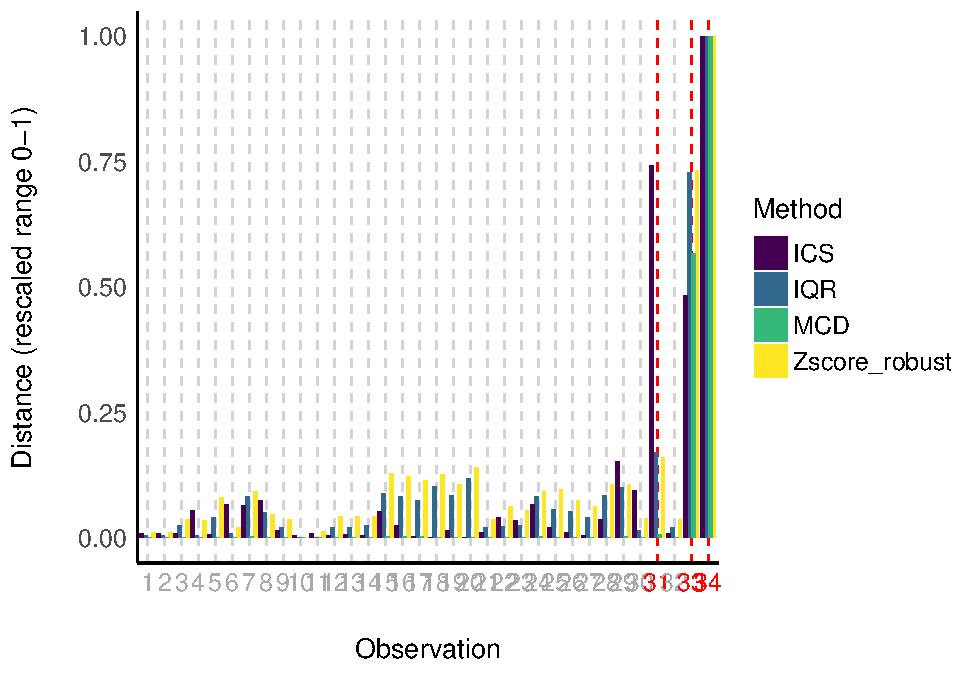
\includegraphics[width=1\linewidth]{paper_files/figure-latex/multimethod-1} \caption{Visual depiction of outliers using several different statistical outlier detection methods.}\label{fig:multimethod}
\end{figure}

An example sentence for reporting the usage of the composite method could be:

\begin{quote}
Based on a composite outlier score (see the `check\_outliers' function in the `performance' R package, Lüdecke et al., 2021) obtained via the joint application of multiple outliers detection algorithms ((a) median absolute deviation (MAD)-based robust z-scores, Leys et al., 2013; (b) interquartile range (IQR), (c) Mahalanobis minimum covariance determinant (MCD), Leys et al., 2019; and (d) invariant coordinate selection (ICS), Archimbaud et al., 2018), we excluded three participants that were classified as outliers by at least half of the methods used.
\end{quote}

\hypertarget{handling-outliers}{%
\section{Handling Outliers}\label{handling-outliers}}

We have at this point demonstrated how to identify outliers. But what should we do with these outliers once identified? Although it is common to automatically discard any observation that has been marked as ``an outlier'' as if it might infect the rest of the data with its statistical ailment, we believe that the use of SOD methods is but one step in the get-to-know-your-data pipeline; a researcher or analyst's \emph{domain knowledge} must be involved in the decision of how to deal with observations marked as outliers by means of SOD. For example, Leys et al. (2019) distinguish between error outliers, interesting outliers, and random outliers.

\emph{Error outliers} are likely due to human error and should be corrected before data analysis or outright removed since they are invalid observations. \emph{Interesting outliers} are not due to technical error and may be of theoretical interest; it might thus be relevant to investigate them further even though they should be removed from the current analysis of interest. \emph{Random outliers} are assumed to be due to chance alone and to belong to the correct distribution and, therefore, should be retained.

It is recommended to \emph{keep} observations which are expected to be part of the distribution of interest, even if they are outliers (Leys et al., 2019). However, if it is suspected that the outliers belong to an alternative distribution, then those observations could have a large impact on the results and call into question their robustness, especially if significance is conditional on their inclusion.

On the other hand, there are also outliers that cannot be detected by statistical tools, but should be found and removed. For example, if we're studying the effects of X on Y among teenagers and we have one observation from a 20-year-old, this observation might not be a \emph{statistical outlier}, but it is an outlier in the \emph{context} of our research, and should be discarded to allow for valid inferences of interest.

\emph{Removing} outliers can in this case be a valid strategy, and ideally one would report results with and without outliers to see the extent of their impact on results. This approach however can reduce statistical power. Therefore, some propose a \emph{recoding} approach, namely, winsorization: bringing outliers back within acceptable limits (e.g., 3 MAD. Tukey \& McLaughlin, 1963). However, if possible, it is recommended to collect enough data so that even after removing outliers, there is still sufficient statistical power without having to resort to winsorization (Leys et al., 2019).

Furthermore, automatic tools can help detect outliers, but they are not perfect. Although they can be useful to flag suspect data, they can have misses and false alarms, and they cannot replace human eyes and proper vigilance from the researcher.

Lastly, we note that no matter which outlier method you use, the handling of outliers should be specified \emph{a priori} with as much detail as possible, and ideally preregistered, to limit researchers' degrees of freedom and therefore risks of false positives (Leys et al., 2019). This is especially true given that interesting outliers and random outliers are oftentimes hard to distinguish in practice. Thus, researchers should always prioritize transparency and report all of the following information: (a) how many outliers were identified; (b) according to which method and criteria, (c) using which function which R package (if applicable), and (d) how they were handled (excluded or winsorized, if the latter, using what threshold). If at all possible, (e) the corresponding code script along with the data should be shared on a public repository like the Open Science Framework, so that the exclusion criteria can be reproduced precisely.

\hypertarget{winsorization}{%
\subsection{Winsorization}\label{winsorization}}

Above, we mentioned a recoding approach to handling outliers: winsorization (Tukey \& McLaughlin, 1963). The \emph{easystats} ecosystem makes it easy to incorporate this step into your workflow through the \texttt{winsorize()} function of the \{datawizard\} package. This procedure will bring back univariate outliers within the limits of `acceptable' values, based either on the percentile, the \emph{z} score, or, ideally, the robust \emph{z} score (based on the MAD).

Example:

\begin{Shaded}
\begin{Highlighting}[]
\NormalTok{data[}\DecValTok{33}\SpecialCharTok{:}\DecValTok{34}\NormalTok{, ]}
\end{Highlighting}
\end{Shaded}

\begin{verbatim}
#>    car mpg cyl disp hp
#> 33  33  42  42   42 42
#> 34  34  55  55   55 55
\end{verbatim}

\begin{Shaded}
\begin{Highlighting}[]
\CommentTok{\# winsorizing using the MAD}
\FunctionTok{library}\NormalTok{(datawizard)}
\NormalTok{winsorized.data }\OtherTok{\textless{}{-}} \FunctionTok{winsorize}\NormalTok{(data, }\AttributeTok{method =} \StringTok{"zscore"}\NormalTok{, }\AttributeTok{robust =} \ConstantTok{TRUE}\NormalTok{, }\AttributeTok{threshold =} \DecValTok{3}\NormalTok{)}

\NormalTok{winsorized.data[}\DecValTok{33}\SpecialCharTok{:}\DecValTok{34}\NormalTok{, ]}
\end{Highlighting}
\end{Shaded}

\begin{verbatim}
#>    car      mpg     cyl disp hp
#> 33  33 37.68598 14.8956   42 42
#> 34  34 37.68598 14.8956   55 55
\end{verbatim}

\hypertarget{conclusion}{%
\section{Conclusion}\label{conclusion}}

In this paper, we have showed how to investigate outliers using the \texttt{check\_outliers()} function of the \{performance\} package while following current good practices. We note that in addition to using the current functions and respecting existing recommendations, it is also important to pre-specify your plans to manage outliers, such as with preregistration, or at the very least justify your choices and stay consistent. Ideally, one would additionally also report the package, function, and threshold used (ideally linking to the full code). We hope that this paper will help more researchers engage in good research practices while providing a smooth outlier detection experience.

\hypertarget{acknowledgments}{%
\section{Acknowledgments}\label{acknowledgments}}

\{performance\} is part of the collaborative \href{https://github.com/easystats/easystats}{\emph{easystats}} ecosystem. Thus, we thank all \href{https://github.com/orgs/easystats/people}{members of easystats}, contributors, and users alike.

\hypertarget{references}{%
\section*{References}\label{references}}
\addcontentsline{toc}{section}{References}

\hypertarget{refs}{}
\begin{CSLReferences}{1}{0}
\leavevmode\vadjust pre{\hypertarget{ref-archimbaud2018ics}{}}%
Archimbaud, A., Nordhausen, K., \& Ruiz-Gazen, A. (2018). ICS for multivariate outlier detection with application to quality control. \emph{Computational Statistics and Data Analysis}, \emph{128}, 184--199. \url{https://doi.org/10.1016/j.csda.2018.06.011}

\leavevmode\vadjust pre{\hypertarget{ref-hubert2018mcd}{}}%
Hubert, M., Debruyne, M., \& Rousseeuw, P. J. (2018). Minimum covariance determinant and extensions. \emph{Wiley Interdisciplinary Reviews: Computational Statistics}, \emph{10}(3), e1421. \url{https://doi.org/10.1002/wics.1421}

\leavevmode\vadjust pre{\hypertarget{ref-leys2019outliers}{}}%
Leys, C., Delacre, M., Mora, Y. L., Lakens, D., \& Ley, C. (2019). How to classify, detect, and manage univariate and multivariate outliers, with emphasis on pre-registration. \emph{International Review of Social Psychology}. \url{https://doi.org/10.5334/irsp.289}

\leavevmode\vadjust pre{\hypertarget{ref-leys2013outliers}{}}%
Leys, C., Ley, C., Klein, O., Bernard, P., \& Licata, L. (2013). Detecting outliers: Do not use standard deviation around the mean, use absolute deviation around the median. \emph{Journal of Experimental Social Psychology}, \emph{49}(4), 764--766. \url{https://doi.org/10.1016/j.jesp.2013.03.013}

\leavevmode\vadjust pre{\hypertarget{ref-ludecke2021performance}{}}%
Lüdecke, D., Ben-Shachar, M. S., Patil, I., Waggoner, P., \& Makowski, D. (2021). {performance}: An r package for assessment, comparison and testing of statistical models. \emph{Journal of Open Source Software}, \emph{6}(60), 3139. \url{https://doi.org/10.21105/joss.03139}

\leavevmode\vadjust pre{\hypertarget{ref-simmons2011false}{}}%
Simmons, J. P., Nelson, L. D., \& Simonsohn, U. (2011). False-positive psychology: Undisclosed flexibility in data collection and analysis allows presenting anything as significant. \emph{Psychological Science}, \emph{22}(11), 1359--1366. \url{https://doi.org/10.1177/0956797611417632}

\leavevmode\vadjust pre{\hypertarget{ref-tukey1963less}{}}%
Tukey, J. W., \& McLaughlin, D. H. (1963). Less vulnerable confidence and significance procedures for location based on a single sample: Trimming/winsorization 1. \emph{Sankhy{ā}: The Indian Journal of Statistics, Series A}, 331--352.

\end{CSLReferences}

\end{document}
